\documentclass[../../../main_physics.tex]{subfiles}

\begin{document}
\renewcommand{\col}{\phy}
\begin{multicols}{2}[\section{Structure of matter and thermodynamics}]
  \subsection{Structure of the matter}
  \subsubsection{Kinetic theory of gases}
  \begin{definition}
    A gas is constituted by large amount of particles moving at higher velocities and satisfying Newton's laws. Hence, we may consider the following assumptions:
    \begin{itemize}
      \item We can underestimate the gravity acting on the particles.
      \item The collisions between particles and between a particle and a wall of the container (perfectly rigid and with infinite mass) are completely elastic.
      \item The particles are point-particles.
      \item There is no interaction between particles (a part from the momentum of a collision).
      \item There is no preferred position and direction for the particles.
    \end{itemize}
  \end{definition}
  \begin{proposition}[Molecular pressure]
    Consider a container of volume $V$ that contains $N$ molecules, each of mass $m$, of a gas. Then, the pressure $P$ of the gas is: $$P=\frac{N}{V}m\langle{v_x}^2\rangle$$ where $\langle{v_x}^2\rangle$ is the mean of the squares of the $x$-components of the velocities of all particles.
  \end{proposition}
  \begin{proposition}[Molecular kinetic energy]
    Consider a gas at a temperature $T$. The average kinetic energy of a particle associated with $x$-axis movement of it is:
    $$\langle K_x\rangle=\frac{1}{2}k_BT$$
    where $k_B$ is the Boltzmann constant. Since, by one of the initial hypothesis, $\langle{v_x}^2\rangle=\langle{v_y}^2\rangle=\langle{v_z}^2\rangle$, then $\langle v^2\rangle=3\langle{v_x}^2\rangle$ and therefore the mean kinetic energy $\langle K\rangle$ of a molecule is: $$\langle K\rangle=\frac{3}{2}k_BT$$
  \end{proposition}
  \begin{proposition}[Molecular velocities]
    Consider a gas of molar mass $M$ constituted by molecules of mass $m$ at a temperature $T$. Then, the \emph{mean-square speed} of the particles is: $$\langle v^2\rangle=\frac{3 k_B T}{m}=\frac{3 R T}{M}$$
    The \emph{root-mean-square speed} is defined as $v_\text{rms}=\sqrt{\langle v^2\rangle}$
  \end{proposition}
  \begin{proposition}[Boltzmann distribution]
    Consider a system at a temperature $T$ in thermodynamic equilibrium. Then, the probability $P(E)$ to find a particle with energy $E$ is proportional to \emph{Boltzmann factor}. That is:
    $$P(E)\propto\exp{-\frac{E}{k_BT}}$$
  \end{proposition}
  \begin{proposition}[Maxwell-Boltzmann distribution]
    The number of molecules (from a total of $N$) of mass $m$ in a gas moving at velocities between $v$ and $v+\dd{v}$ and at a temperature $T$ is:
    $$\dd{N}=Nf(v)\dd{v}$$ where $f(v)$ is: $$f(v)=\frac{4}{\sqrt{\pi}}{\left(\frac{m}{2k_BT}\right)}^{3/2}v^2\exp{-\frac{mv^2}{2k_BT}}$$
  \end{proposition}
  \begin{proposition}[Distribution of molecular velocities]
    Consider a gas constituted of molecules of mass $m$ moving at a velocity $v$ at a temperature $T$. If $v_\text{max}$, $\langle v\rangle$ and $v_\text{rms}$ are the maximum speed, mean speed and root-mean-square speed respectively, then:
    \begin{gather*}
      \dv{f(v)}{v}=0\implies v_\text{max}=\sqrt{\frac{2k_BT}{m}}\\
      \langle v\rangle=\int_0^\infty vf(v)\dd{v}=\sqrt{\frac{8k_BT}{\pi m}}\\
      v_\text{rms}=\sqrt{\langle v^2\rangle}=\sqrt{\int_0^\infty v^2f(v)\dd{v}}=\sqrt{\frac{3k_BT}{m}}
    \end{gather*}
  \end{proposition}
  \subsubsection{Specific heat and equipartition theorem}
  \begin{definition}
    When we heat up a substance, we transfer energy to it resulting in an increase of its internal energy $U$. The amount of heat $Q$ necessary to increase the temperature of a substance is proportional to the variation of the temperature and its mass $m$. That is:
    $$Q=C\Delta T=cm\Delta T$$
  \end{definition}
  \begin{definition}
    \emph{Heat capacity} $C$ is defined as the amount of heat to be supplied to an object to increase its temperature by one degree.
  \end{definition}
  \begin{definition}
    \emph{Specific heat} $c$ is defined as the heat capacity per unit of mass: $$c=\frac{C}{m}$$ where $m$ is the mass of the object to heat.
  \end{definition}
  \begin{definition}
    \emph{Molar heat capacity} $c_\text{m}$ is defined as the heat capacity per unit of mole: $$c_\text{m}=\frac{C}{n}=\frac{mc}{n}=\frac{M}{n}$$ where $n$ is the number of moles of the object to heat, $m$ its mass and $M$ its molar mass.
  \end{definition}
  \begin{definition}
    The \emph{adiabatic index} $\gamma$ is defined as:
    $$\gamma=\frac{C_P}{C_V}$$
    where $C_P$ is the heat capacity at constant pressure and $C_V$ is the heat capacity at constant volume\footnote{In liquids and solids we have $C_p\approx C_V=:C$.}.
  \end{definition}
  \begin{definition}[Internal energy]
    The internal energy $U$ of an ideal gas constituted of monoatomic particles is:
    $$U=N\langle K_\text{trans}\rangle=\frac{3}{2}nRT$$
    where $N$ is the number of particles in the gas on it; $n$, the number of moles, and $T$, its the temperature.
  \end{definition}
  \begin{proposition}[Mayer's relation]
    Consider a substance constituted by $n$ moles of an ideal gas. Then:
    $$C_P=C_V+nR$$
  \end{proposition}
  \begin{proposition}[Heat capacities in gases]
    Consider a substance constituted by $n$ moles of an ideal gas. Since $C_V=\dv{U}{T}$, we have: $$C_V=\frac{3}{2}nR\qquad C_P=\frac{5}{2}nR$$ Therefore, $\gamma=\frac{5}{3}$.
  \end{proposition}
  \begin{theorem}[Equipartition theorem]
    Consider a substance at a temperature $T$ in thermodynamic equilibrium. Then, the energy behave equally in each quadratic degree of freedom associated at each component of the kinetic or potential energy. Thus, there exists an average energy of $\frac{1}{2}k_BT$ per molecule or an average energy of $\frac{1}{2}RT$ per mole associated with each degree of freedom\footnote{The equipartition theorem fails when temperatures are very high or very low due to the discretization of the energy postulated by quantum physics.}.
  \end{theorem}
  \begin{corollary}[Equipartition theorem on diatomic molecules]
    Consider a diatomic molecule of mass $m$ rotating around $x$ and $y$ axis. Then, its energy will be of the form:
    $$E=\frac{1}{2}m\left({v_x}^2+{v_y}^2+{v_z}^2\right)+\frac{1}{2}I_x{\omega_x}^2+\frac{1}{2}I_y{\omega_y}^2$$
    Since we have 5 quadratic degrees of freedom, the total energy $E$ will be $E=\frac{5}{2}k_BT$. If a gas in constituted by $N$ diatomic molecules, then:
    $$U=NE=\frac{5}{2}Nk_BT=\frac{5}{2}nN_Ak_BT=\frac{5}{2}nRT$$ where $N_A$ is the Avogadro constant and $n$ is the number of moles of the gas. Therefore, we will have $C_V=\frac{5}{2}nR$, $C_P=\frac{7}{2}nR$ and $\gamma=\frac{7}{5}$.
  \end{corollary}
  \begin{corollary}[Dulong-Petit law]
    Consider a solid and suppose its atoms are connected with springs with effective constant $k_\text{eff}$. Then:
    $$E=\frac{1}{2}m\left({v_x}^2+{v_y}^2+{v_z}^2\right)+\frac{1}{2}k_\text{eff}\left(x^2+y^2+z^2\right)$$
    Since we have 6 quadratic degrees of freedom, the total energy $E$ will be $E=\frac{6}{2}k_BT$. If a gas in constituted by $N$ atoms, then:
    $$U=NE=\frac{6}{2}Nk_BT=3nN_Ak_BT=3nRT$$ where $n$ is the number of moles of the solid. Therefore, we will have $C=3nR$.
  \end{corollary}
  \subsubsection{Black-body radiation}
  \begin{definition}[Thermal radiation]
    \emph{Thermal radiation} is the electromagnetic radiation emitted by a body as a consequence of its temperature. All bodies emit this radiation and absorb the one emitted by its surroundings. In thermal equilibrium the emission and absorption are equal.
  \end{definition}
  \begin{proposition}[Black body]
    A \emph{black body} is an object that absorbs all electromagnetic radiation incident on it.
  \end{proposition}
  \begin{proposition}[Stefan-Boltzmann law]
    The energy radiated by a black body at a temperature $T$ per unit of area and time (called \emph{radiance}) is: $$I=\sigma T^4$$ where $\sigma$ is the Stefan-Boltzmann constant.
  \end{proposition}
  \begin{proposition}[Wien's displacement law]
    The radiance does not distribute uniformly along all wavelengths (\emph{spectral radiance} $I(\lambda)$). The maximum of this function is taken when $$\lambda_\text{max}=:\frac{b}{T}$$ where $b$ is the \emph{Wien's displacement constant} and $T$ is the temperature of the body.
  \end{proposition}
  \begin{proposition}[Rayleigh-Jeans law]
    \emph{Rayleigh-Jeans law} is an approximation to the spectral radiance of electromagnetic radiation of a black body at a given temperature $T$ as a function of the wavelength through classical arguments: $$I(\lambda)=\frac{2\pi c k_B T}{\lambda^4}\footnote{The Rayleigh-Jeans law agrees with experimental results at large wavelengths (low frequencies) but strongly disagrees at short wavelengths (high frequencies). This inconsistency between observations and the predictions of classical physics is commonly known as the \emph{ultraviolet catastrophe}.}$$
  \end{proposition}
  \begin{proposition}[Planck's law]
    To solve the ultraviolet catastrophe, Planck deduced the following formula for the spectral radiance: $$I(\lambda)=\frac{2\pi h c^2}{\lambda^5\left(\exp{\frac{hc}{\lambda k_B T}}-1\right)}\footnote{Note that from here we can deduced Stefan-Boltzmann and Wien's displacement laws as follows: $$I=\int_0^\infty I(\lambda)\dd\lambda=\frac{2\pi^5 {k_B}^4}{15c^2h^3}T^4=:\sigma T^4\qquad \dv{I(\lambda)}{\lambda}=0\implies\lambda=\frac{hc}{4.965}\cdot\frac{1}{T}=:\frac{b}{T}$$}$$
  \end{proposition}
  \begin{center}
    \begin{minipage}{\linewidth}
      \centering
      \includestandalone[mode=image|tex,width=\linewidth]{Images/ultraviolet_catastrophe}
      \captionof{figure}{Graphical illustration of the ultraviolet catastrophe}
    \end{minipage}
  \end{center}
  \subsubsection{Photoelectric effect}
  \begin{definition}[Photoelectric effect]
    The \emph{photoelectric effect} consists in the emission of electrons when electromagnetic radiation hits a material. Electrons emitted in this manner are called \emph{photoelectrons}. Moreover we have the following properties:
    \begin{itemize}
      \item Photoelectric effect only occurs when the incident light is of frequency greater than or equal to a \emph{threshold frequency} $\nu_0$.
      \item Kinetic energy of the electrons increase proportionally to the frequency of the incident light.
      \item Increasing the intensity of the incident light does not increase the energy of photoelectrons, but the number of photoelectrons.
    \end{itemize}
  \end{definition}
  \begin{proposition}[Stopping potential]
    Let $\phi$ be the energy required to remove an electron from the surface of a material. If we hit this surface with photons of frequency $\nu$, then: $$\frac{1}{2}m_e{v_\text{max}}^2=h\nu-\phi$$ Moreover, if we connect a potential difference $V$ contrary to the movement of the electrons, then: $$eV=h\nu-\phi$$ The electrons with lower energy than $\phi=h\nu_0$ won't have enough energy to remove an electron of the material.
  \end{proposition}
  \begin{proposition}[Planck-Einstein relation]
    Relating the energy $E$ of a photon of frequency $\nu$ and wavelength $\lambda$ we have: $$E=h\nu=\frac{hc}{\lambda}$$
  \end{proposition}
  \begin{proposition}[De Broglie relation]
    The momentum $p$ of photons of energy $E$ and wavelength $\lambda$ is: $$p=\frac{E}{c}=\frac{h}{\lambda}$$
  \end{proposition}
  \subsubsection{Light}
  \begin{definition}[Light]
    We can think the light as a particle or as a wave. In particular, when it propagates, it behave like an electromagnetic wave and travels at a velocity $$c=\frac{1}{\sqrt{\varepsilon_0\mu_0}}$$ where $\varepsilon_0$ is the vacuum permittivity and $\mu_0$ vacuum permeability. Moreover the oscillating directions of the electric and magnetic field are perpendicular to each other and to the direction of propagation.
  \end{definition}
  \begin{definition}[Compton scattering]
    The \emph{compton scattering} occurs when a photon of wavelength $\lambda_1$ collides with an electron and as a consequence the collision produces another photon of wavelength $\lambda_2>\lambda_1$ (with less energy than the pervious one) deflected an angle $\theta$ from the original trajectory of the photon. Moreover, we have:
    $$\lambda_2-\lambda_1=\frac{h}{m_ec}(1-\cos\theta)\footnote{This is deduced taking into account the conservation of energy and momentum.}$$
    where $m_e$ is the mass of the electron.
  \end{definition}
  \subsubsection{Matter wave}
  \begin{proposition}[Bohr's complementary principle]
    There are experiments in which bodies behave like particles and other ones in which they behave like waves.
  \end{proposition}
  \begin{definition}[Wavelenth of a particle]
    Consider a particle of mass $m$, kinetic energy $K$ and momentum $p$. Then its wavelength is: $$\lambda=\frac{h}{p}=\frac{hc}{2mc^2K}$$ As a consequence, all elementary particles propagate like waves an exchange energy like particles.
  \end{definition}
  \begin{proposition}[Heisenberg's uncertainty principle]
    Let $\Delta Y$ be the uncertainty of the magnitude $Y$ of a particle. Then, for all particles we have: $$\Delta x\Delta p\geq\frac{\hbar}{2}\qquad\Delta E\Delta t\geq\frac{\hbar}{2}$$
  \end{proposition}
  \subsubsection{Wave function}
  \begin{definition}[Schrödinger equation]
    Given that we cannot know the position and velocity of a particle with unlimited precision, a particle of mass $m$ is described with a \emph{wave function} $\Psi(x,t)$\footnote{It is important that the function $\Psi(x,t)$ must be continuous.} which is a solution to \emph{Schrödinger equation}:
    $$\frac{-\hbar^2}{2m}\pdv[2]{\Psi(x,t)}{x}+U(x,t)\Psi(x,t)=\ii\hbar\pdv{\Psi(x,t)}{t}$$
    where $U(x,t)$ is the potential energy that the particle is subject to. More generally, the Schrödinger equation in three dimensions is:
    $$\frac{-\hbar^2}{2m}\laplacian\Psi(\vf{r},t)+U(\vf{r},t)\Psi(\vf{r},t)=\ii\hbar\pdv{\Psi(\vf{r},t)}{t}$$ where $\vf{r}=x\vf{i}+y\vf{j}+z\vf{k}$.
  \end{definition}
  \begin{proposition}[Properties of Schrödinger equation]
    Consider a particle whose wave function is $\Psi(x,t)$. Then:
    \begin{itemize}
      \item The probability to find the particle between $x$ and $x+\dd{x}$ is: $$|\Psi(x,t)|^2\dd{x}$$
      \item \emph{Probability density}: $$P(x,t)=|\Psi(x,t)|^2=\Psi(x,t)\Psi^*(x,t)$$
      \item \emph{Normalization condition}: $$\int_{-\infty}^\infty|\Psi(x,t)|^2\dd{x}=1$$
      \item \emph{Expectation value} of $x$: $$\langle x\rangle=\int_{-\infty}^\infty x\Psi(x,t)\Psi^*(x,t)\dd{x}=1$$
    \end{itemize}
    Here $\Psi^*(x,t)$ denotes the complex conjugate of $\Psi(x,t)$.
  \end{proposition}
  \begin{definition}[Time-independent Schrödinger equation]
    Consider a stationary solution of the Schrö\-din\-ger equation of the form: $$\Psi(x,t)=\Phi(x)\exp{\frac{-\ii Et}{\hbar}}$$
    Then, if the potential energy $U(x,t)$ to which the particle is subject does not depend on time, that is $U(x,t)=U(x)$, we get the \emph{time-independent Schrödinger equation}:
    \begin{equation}\label{SMT_schrodinger}
      \frac{-\hbar^2}{2m}\dv[2]{\Phi(x)}{x}+U(x)\Phi(x)=E\Phi(x)
    \end{equation}
  \end{definition}
  \begin{proposition}[Particle in a box-1D]
    Consider a particle of mass $m$ confined in a 1-dimensional box of length $L$. We can think that it is subjected to a potential $$U(x)=
      \begin{cases}
        \infty & \text{if }x\leq 0   \\
        0      & \text{if }0 < x < L \\
        \infty & \text{if }x\geq L   \\
      \end{cases}
    $$
    Since the particle cannot leave the region $(0,L)$, we have that $\Phi(x)=0$ for $x\leq 0$ and $x\geq L$. Therefore, by \cref{SMT_schrodinger}:
    $$
      \frac{-\hbar^2}{2m}\dv[2]{\Phi(x,t)}{x}=E\Phi(x)\qquad\text{for }0\leq x\leq L
    $$
    If we define $k^2=\frac{2m E}{\hbar^2}$, we have
    $$
      \dv[2]{\Phi(x,t)}{x}+k^2\Phi(x)=0\qquad\text{for }0\leq x\leq L
    $$
    which is the equation of a simple harmonic oscillator with solution $\Phi(x)=A\sin(kx)+B\cos(kx)$. Taking into account boundary conditions, we have that: $$\Phi(x)=\Phi_n(x)=\sqrt{\frac{2}{L}}\sin\left(\frac{n\pi}{L}x\right)$$ where the number $n\in\NN$ is called \emph{quantum number}. In particular, $k=k_n=\frac{n\pi}{L}$ and therefore: $$E_n=\frac{\hbar^2k_n^2}{2m}=n^2\left(\frac{h^2}{8mL^2}\right)=n^2E_1$$ And we observe that the energy is discretized in different levels.
  \end{proposition}
  \begin{proposition}[Particle in a box-3D]
    If the particle of mass $m$ is now confined to a three-dimensional box of edges $a$, $b$ and $c$, we get:
    $$\Phi_{n_xn_yn_z}(\vf{r})=\sqrt{\frac{8}{abc}}\sin\left(\frac{n_x\pi}{a}x\right)\sin\left(\frac{n_y\pi}{b}x\right)\sin\left(\frac{n_z\pi}{c}x\right)$$
    where $n_x$, $n_y$ and $n_z$ are independent quantum numbers\footnote{This is obtained from the fact that the solutions $\Phi{n_xn_yn_z}(\vf{r})$ of the Schrödinger equation in three dimensions are of the form: $\Phi{n_xn_yn_z}(\vf{r})=\Phi_{n_x}(x)\Phi_{n_y}(y)\Phi_{n_z}(z)$}. Moreover:
    $$E_{n_xn_yn_z}={n_x}^2\left(\frac{h^2}{8ma^2}\right)+{n_y}^2\left(\frac{h^2}{8mb^2}\right)+{n_z}^2\left(\frac{h^2}{8mc^2}\right)$$
  \end{proposition}
  \begin{definition}
    An energy level is \emph{degenerate} if it corresponds to two or more different measurable states of a quantum system. For example, if a particle is contained in a cube, then: $$E_{112}=E_{121}=E_{211}=6E_1$$ where $E_1$ is the ground-state energy of the particle contained in a 1-dimensional box.
  \end{definition}
  \begin{proposition}[Bohr's correspondence principle]
    In the limit of very large quantum numbers, the classical calculation and the quantum calculation must yield the same results.
  \end{proposition}
  \subsubsection{Atoms}
  \begin{definition}[Bohr model]
    The Bohr model\footnote{Bohr model only works for monoelectronic atoms, that is, atoms with only one electron.} of an atom can be sum up with three postulates:
    \begin{enumerate}
      \item The electrons can move only in certain non-radiating circular orbits called stationary states.
      \item If $E_i$ and $E_f$ are the initial and final energies of the atom, the frequency of the emitted radiation during a transition is given by $$\nu=\frac{E_i-E_f}{h}$$
      \item The angular momentum is quantized: $$m_ev_nr_n=n\hbar\qquad n\in\NN$$ where $v_n$ and $r_n$ are the speed of the electron and the radius of the orbit respectively in the state $n$.
    \end{enumerate}
  \end{definition}
  \begin{proposition}[Radii of Bohr orbits]
    The radius $r_n$ of the $n$-th Bohr orbit of a monoelectronic atom with atomic number $Z$ is: $$r_n=n^2\frac{\hbar^2}{m_ekZe^2}=:n^2\frac{a_0}{Z}$$
    where $k$ is the Coulomb constant. $a_0=0.0529\text{ nm}$ is called \emph{first Bohr radius}.
  \end{proposition}
  \begin{proposition}[Energy levels]
    The total energy $E_n$ of the $n$-th orbit of a monoelectronic atom with atomic number $Z$ is is:
    \begin{equation}\label{SMT_energy-levels}
      E_n=-Z^2\frac{E_0}{n^2}
    \end{equation}
    where $E_0=\frac{m_ek^2e^4}{2\hbar^2}=13.6\text{ eV}$.
  \end{proposition}
  \begin{proposition}[Rydberg-Ritz law]
    An electron that goes from an energy level $n_i$ to a lower one $n_f<n_i$ emits a photon whose wavelength is:
    $$\frac{1}{\lambda}=\frac{k^2m_ee^4}{4\pi c\hbar^3}Z^2\left(\frac{1}{{n_f}^2}-\frac{1}{{n_i}^2}\right)=:R_HZ^2\left(\frac{1}{{n_f}^2}-\frac{1}{{n_i}^2}\right)$$
    where $R_H$ is the \emph{Rydberg constant}.
  \end{proposition}
  \subsubsection{Quantum theory of atoms}
  \begin{definition}[Quantum numbers in spherical coordinates]
    Consider an atom with a single electron. Then, the potential energy for the electron depends only on the radial component and so we can make a change of variable to spherical coordinates $(r,\theta,\phi)$\footnote{Here $\phi$ denotes the azimuthal angle.}. Hence, the independent quantum numbers $n_x$, $n_y$ and $n_z$ obtained from Cartesian coordinates will become the quantum numbers $n$ (associated with $r$), $\ell$ (associated with $\theta$) and $m_\ell$\footnote{Sometimes for simplicity the subindex $\ell$ is omitted.} (associated with $\phi$), which in this case, are not independent. More precisely we have:
    \begin{itemize}
      \item \emph{Principal quantum number}: $n=1,2,3,\ldots$\par
            The energy, as seen in \cref{SMT_energy-levels}, is given by: $$E_n=-Z^2\frac{13.6\text{ eV}}{n^2}$$
      \item \emph{Orbital quantum number}: $\ell=0,1,2,\ldots,n-1$\par Moreover the magnitude $\|\vf{L}\|$ of the orbital angular momentum $\vf{L}$ is related to the orbital quantum number $\ell$ by: $$\|\vf{L}\|=\sqrt{\ell(\ell+1)}\hbar$$
      \item \emph{Magnetic quantum number}: $m_\ell=0,\pm 1,\pm 2,\ldots,\pm\ell$\par
            Moreover the $z$ component $L_z$ of the orbital angular momentum $\vf{L}$ is given by the quantum condition $$L_z=m_\ell\hbar$$
    \end{itemize}
    Therefore are $n^2$ degenerate states for the energy $E_n$.
    In terms of wave function we can write $$\Psi_{n\ell m_\ell}(\vf{r})=R_{n\ell}(\vf{r})Y_{\ell m_\ell}(\vf{r})$$
  \end{definition}
  \begin{definition}[Spin]
    An electron has a \emph{intrinsic orbital angular momentum} or simply \emph{spin} $\vf{S}$ such that:
    $$\|\vf{S}\|=\sqrt{s(s+1)}\hbar\qquad S_z=s\hbar$$ where $s=\pm\frac{1}{2}$ is another quantum number  to be considered in the wave function and it is called \emph{spin quantum number}. This fact result in $2n^2$ possible states for the energy $E_n$ of an electron.
  \end{definition}
  \begin{center}
    \begin{minipage}{\linewidth}
      \centering
      \begin{tabular}{cccl}
        \hline
        \hline
        $n$ & $\ell$ & Type of orbital & $m_\ell$                              \\
        \hline
        1   & 0      & $s$             & 0                                     \\
            &        &                 &                                       \\
        2   & 0      & $s$             & 0                                     \\
        2   & 1      & $p$             & $-1$, 0, 1                            \\
            &        &                 &                                       \\
        3   & 0      & $s$             & 0                                     \\
        3   & 1      & $p$             & $-1$, 0, 1                            \\
        3   & 2      & $d$             & $-2$, $-1$, 0, 1, 2                   \\
            &        &                 &                                       \\
        4   & 0      & $s$             & 0                                     \\
        4   & 1      & $p$             & $-1$, 0, 1                            \\
        4   & 2      & $d$             & $-2$, $-1$, 0, 1, 2                   \\
        4   & 3      & $f$             & $-3$, $-2$, $-1$, 0, 1, 2, 3          \\
            &        &                 &                                       \\
        5   & 0      & $s$             & 0                                     \\
        5   & 1      & $p$             & $-1$, 0, 1                            \\
        5   & 2      & $d$             & $-2$, $-1$, 0, 1, 2                   \\
        5   & 3      & $f$             & $-3$, $-2$, $-1$, 0, 1, 2, 3          \\
        5   & 4      & $g$             & $-4$, $-3$, $-2$, $-1$, 0, 1, 2, 3, 4 \\
        \hline
        \hline
      \end{tabular}
      \captionof{table}{Atomic orbitals in terms of quantum numbers $n$, $\ell$ and $m_\ell$. Moreover for each configuration we have two possible values for the spin: $-\frac{1}{2}$ and $\frac{1}{2}$.}
    \end{minipage}
  \end{center}
  \subsubsection{Polyelectronic atoms}
  \begin{proposition}[Schrödinger equation]
    Consider an atom with $N$ electrons. The Schrödinger equation becomes:
    \begin{multline*}
      \left\{\frac{-\hbar}{2\mu}\sum_{i=1}^N{\grad_i}^2-\sum_{i=1}^N\frac{Ze^2}{4\pi\varepsilon_0r_i}+\sum_{\substack{i,j=1\\i>j}}^N\frac{e^2}{4\pi\varepsilon_0r_{ij}}\right\}\cdot\\\cdot\Phi(\vf{r}_1,\ldots,\vf{r}_N)=E\Phi(\vf{r}_1,\ldots,\vf{r}_N)
    \end{multline*}
    where $\displaystyle\mu=\frac{m_\text{nuc}m_e}{m_\text{nuc}+m_e}$ is the reduced mass of the electron ($m_e$) and the nucleus ($m_\text{nuc}$), $\vf{r}_i=x_i\vf{i}+y_i\vf{j}+z_i\vf{k}$ and $\displaystyle{\grad_i}^2=\pdv[2]{}{x_i}+\pdv[2]{}{y_i}+\pdv[2]{}{z_i}$.
    This equation cannot be solved exactly but we can find approximations to it if we suppose:
    \begin{itemize}
      \item We neglect the interactions between electrons.
      \item We consider that the particles are identic and we cannot distinguish them.
    \end{itemize}
  \end{proposition}
  \begin{definition}[Fermions]
    A \emph{fermion} is a particle that follows Fermi-Dirac statistics and has half integer spin.
  \end{definition}
  \begin{definition}[Boson]
    A \emph{boson} is a particle that follows Bose-Einstein statistics and has integer spin.
  \end{definition}
  \begin{proposition}[Pauli exclusion principle]
    Two or more identical fermions cannot occupy simultaneously the same quantum state.
  \end{proposition}
  \begin{proposition}[Symmetry of the wave function]
    Consider two non-interacting identical particles. The probability density of the two particles with wave function $\Psi(\vf{r}_1,\vf{r}_2)$ must be identical to that with wave function $\Psi(\vf{r}_2,\vf{r}_1)$. Therefore, $${|\Psi(\vf{r}_1,\vf{r}_2)|}^2={|\Psi(\vf{r}_2,\vf{r}_1)|}^2$$ and hence $\Psi$ has to be necessary symmetric ($\Psi(\vf{r}_1,\vf{r}_2)=\Psi(\vf{r}_2,\vf{r}_1)$) or antisymmetric ($\Psi(\vf{r}_1,\vf{r}_2)=-\Psi(\vf{r}_2,\vf{r}_1)$). Moreover we have:
    \begin{enumerate}
      \item $\Phi$ is symmetric if and only if the particles are bosons.
      \item $\Phi$ is antisymmetric if and only if the particles are fermions.
    \end{enumerate}
  \end{proposition}
  \subsubsection{Nuclear physics}
  \begin{definition}[Atom]
    An atom X formed by $Z$ protons and $N$ neutrons is denoted as \ce{^A_ZX} where $A:=Z+N$\footnote{Sometimes if the atom \ce{^A_ZX} is well-known, we simply refer to it as \ce{^AX}.}. The number $Z$ is called \emph{atomic number} and the number $A$, \emph{mass number}.
  \end{definition}
  \begin{definition}
    Two nuclides are
    \begin{itemize}
      \item \emph{isotopes} if they have the same $Z$ but different $N$ and $A$.
      \item \emph{isobars} if they have the same $N$ but different $Z$ and $A$.
      \item \emph{isotones} if they have the same $A$ but different $Z$ and $N$.
      \item \emph{isomers} if they have the same $Z$, $N$ and $A$. They differ in the grouping structure.
    \end{itemize}
  \end{definition}
  \begin{proposition}[Radii of nucleus]
    The stable nucleus has approximately constant density and therefore the nuclear radius $R$ can be approximated by the following formula:
    $$R=R_0A^{1/3}$$ where $R_0\approx1.2\text{ fm}$.
  \end{proposition}
  \begin{proposition}[Nucleus mass]
    The mass of a nucleus $M_\text{nuc}(Z,A)$ of atomic number $Z$ and mass number $A$ satisfies:
    $$M_\text{nuc}(Z,A)c^2=Zm_\text{p}c^2+(A-Z)m_\text{n}c^2-E_\text{b}(Z,A)$$ where $E_\text{b}(Z,A)$ is the \emph{binding energy}, that is, the energy required to break up the nucleus into $Z$ protons and $A-Z$ neutrons. If we take into account the mass of the electrons on the atomic mass $M_\text{at}(Z,A)$ we get:
    \begin{multline*}
      M_\text{at}(Z,A)c^2=M_\text{nuc}(Z,A)c^2+Zm_ec^2-E_e(Ze)\approx\\\approx ZM_\text{at}(\ce{^1_1H})c^2+(A-Z)m_\text{n}c^2-E_\text{b}(Z,A)
    \end{multline*}
    where $E_e(Ze)$ is the \emph{electron binding energy} and $E_e(Ze)\ll E_\text{b}(Z,A)$ so it can be neglected, and $M_\text{at}(\ce{^1_1H})$ is the mass of hydrogen atom \ce{^1_1H}. From this, we can define the \emph{mass defect} $\Delta m$:
    $$\Delta m=M_\text{at}(Z,A)-A$$ where $M_\text{at}(Z,A)$ is expressed in u\footnote{Unified atomic mass unit.}.
  \end{proposition}
  \begin{center}
    \begin{minipage}{\linewidth}
      \centering
      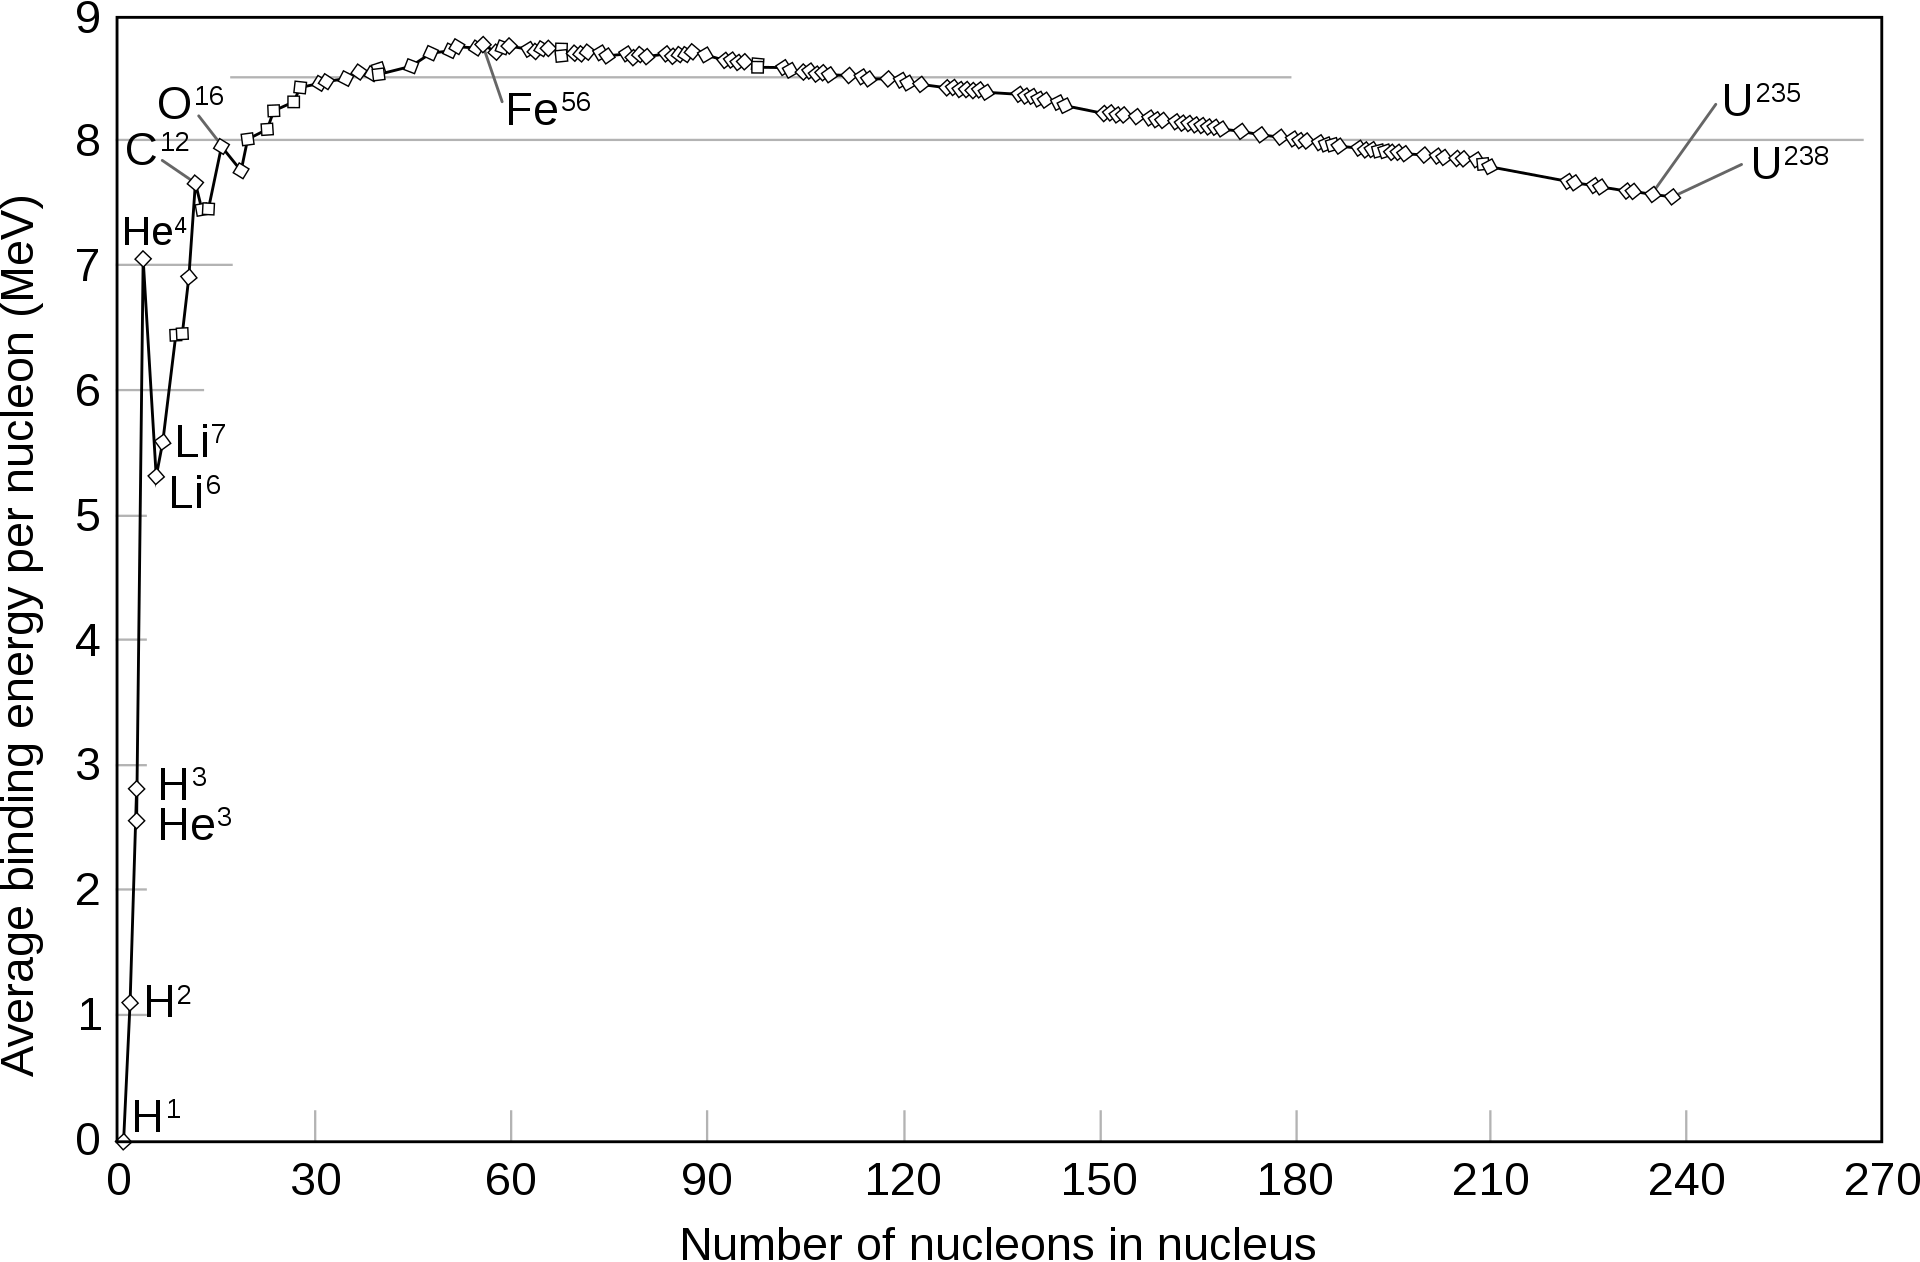
\includegraphics[width=\linewidth]{Images/Binding_energy.png}
      \captionof{figure}{Binding energy curve}
    \end{minipage}
  \end{center}
  \begin{proposition}[Semi-empirical mass formula]
    For a nucleus of atomic number $Z$ and mass number $A$, we have:
    \begin{multline*}
      E_\text{b}(Z,A)=c_1A-c_2A^{2/3}-c_3\frac{Z(Z-1)}{A^{1/3}}-\\-c_4\frac{{(2Z-A)}^2}{A}+\delta(Z,A)
    \end{multline*}
    where
    $$\delta(Z,A)=
      \begin{cases}
        -c_5A^{-1/2} & \text{if }N, Z\text{ are odd}  \\
        0            & \text{if }A\text{ is odd}      \\
        +c_5A^{-1/2} & \text{if }N, Z\text{ are even} \\
      \end{cases}
    $$
    empirically, it can be seen that $c_1\approx 15.56\text{ MeV}$, $c_2\approx 17.23\text{ MeV}$, $c_3\approx 0.697\text{ MeV}$, $c_4\approx 23.285\text{ MeV}$ and $c_1\approx 12.00\text{ MeV}$.
  \end{proposition}
  \begin{definition}[Q value]
    The \emph{$Q$ value} for a reaction is defined as: $$Q=(m_i-m_f)c^2$$ where $m_i$ is the sum of the reactant masses and $m_f$ is the sum of the product masses. The decay will be spontaneous if $Q>0$ and in this case, the decay will have a net release of energy.
  \end{definition}
  \begin{definition}[$\alpha$-decay]
    An $\alpha$ particle is a nucleus of \ce{^4_2He}, which has a short range.
    The decay is: $$\ce{^$A$_$Z$X}\rightarrow\ce{^$A-4$_$Z-2$Y}+\alpha$$
    In this case:
    \begin{multline*}
      Q=\left[M_\text{nuc}\left(\ce{^$A$_$Z$X}\right)-M_\text{nuc}\left(\ce{^$A-4$_$Z-2$Y}\right)-M_\text{nuc}\left(\ce{^4_2He}\right)\right]c^2=\\=\left[M_\text{at}\left(\ce{^$A$_$Z$X}\right)-M_\text{at}\left(\ce{^$A-4$_$Z-2$Y}\right)-M_\text{at}\left(\ce{^4_2He}\right)\right]c^2=\\=K_Y+K_\alpha
    \end{multline*}
    where $M_\text{at}\left(\ce{^$A$_$Z$X}\right)$ is the mass of the atom \ce{^4_2X}, $M_\text{nuc}\left(\ce{^$A$_$Z$X}\right)$ is the mass of its nucleus (and the same for the atom Y), $K_\text{Y}$ is the kinetic energy of the particle Y and $K_\alpha$ is the kinetic energy of the $\alpha$ particle. Moreover we have: $$K_\text{Y}\approx \frac{4}{A}Q\qquad K_\alpha\approx \frac{A-4}{A}Q$$
  \end{definition}
  \begin{definition}[$\beta$-decay]
    \hfill
    \begin{enumerate}
      \item \emph{$\beta^-$ decay}: $\text{n}\rightarrow\text{p}+e^-+\bar{\nu}_e$\par
            The decay: $$\ce{^$A$_$Z$X}\rightarrow\ce{^$A$_$Z+1$Y}+e^-+\bar{\nu}_e$$
            $Q$ factor\footnote{Since neutrino's mass is around 2 eV, we can neglect it.}: $$Q=\left[M_\text{at}\left(\ce{^$A$_$Z$X}\right)-M_\text{at}\left(\ce{^$A$_$Z+1$Y}\right)\right]c^2$$
      \item \emph{$\beta^+$ decay}: $\text{p}\rightarrow\text{n}+e^++\nu_e$\par
            The decay: $$\ce{^$A$_$Z$X}\rightarrow\ce{^$A$_$Z-1$Y}+e^++\nu_e$$
            $Q$ factor: $$Q=\left[M_\text{at}\left(\ce{^$A$_$Z$X}\right)-M_\text{at}\left(\ce{^$A$_$Z-1$Y}\right)-2m_e\right]c^2$$
      \item \emph{Electron capture}: $\text{p}+e^-\rightarrow\text{n}+\nu_e$\par
            The decay: $$\ce{^$A$_$Z$X}+e^-\rightarrow\ce{^$A$_$Z-1$Y}+\nu_e$$
            $Q$ factor: $$Q=\left[M_\text{at}\left(\ce{^$A$_$Z$X}\right)-M_\text{at}\left(\ce{^$A$_$Z-1$Y}\right)\right]c^2-B_n$$
            where $B_n$ is the ionization energy at the shell $n$ where the electron is captured.
    \end{enumerate}
  \end{definition}
  \begin{definition}[$\gamma$-decay]
    A $\gamma$ particle is a photon which has long range. The decay is produced when the nucleus goes from an excited state to a less excited state. The decay is: $$\ce{^$A$_$Z$X}^*\rightarrow\ce{^$A$_$Z$X}+\gamma$$
  \end{definition}
  \begin{definition}[Radioactive activity]
    The \emph{radioactive activity} of a substance is defined as the number of decays it has per unit of time. Its unit in the SI is the Bq ($[\text{Bq}]=[\text{s}^{-1}]$). The probability for a radionuclide to decay per unit of time is constant and unique for each radionuclide. This constant $\lambda$ is called \emph{decay constant}. Moreover if $N(t)$ is the number of radionuclide to decay at time $t$ and $A(t)$ is the activity of the substance at time $t$, we have:
    $$A(t)=\lambda N(t)=-\dv{N(t)}{t}$$ And therefore:
    $$N(t)=N_0\exp{-\lambda t}\qquad A(t)=A_0\exp{-\lambda t}$$
    where $N_0$ is the initial number of radionuclides and $A_0=\lambda N_0$ is the initial activity of the substance.
  \end{definition}
  \begin{definition}[Half-time]
    We define the \emph{half-time} $t_{1/2}$ as the time in which the number of radionuclide has reduced by half.
  \end{definition}
  \begin{center}
    \begin{minipage}{\linewidth}
      \centering
      \includestandalone[mode=image|tex,width=1\linewidth]{Images/thorium_series}
      \captionof{figure}{Decay chain of Thorium or \emph{Thorium series} corresponding to nuclei with $A=4n$, $n\in\NN$.}
    \end{minipage}
  \end{center}
  \begin{proposition}[Decay chain]
    Consider the decay chain:
    \begin{center}
      \begin{minipage}{\linewidth}
        \centering
        \includestandalone[mode=image|tex,width=0.75\linewidth]{Images/decay_chain}
      \end{minipage}
    \end{center}
    where the third nucleus is stable.
    Let $N_i(t)$ be the number of radionuclides of the substance $i$ at time $t$, $A_i(t)$ be the activity of the substance $i$ at time $t$ and $\lambda_i$ be the decay constance of the substance $i$, all of this for $i=1,2$. Then, if $N_1(0)=N_0$ and $N_2(0)=N_3(0)=0$, we have:
    \begin{gather*}
      N_1(t)=N_0\exp{-\lambda_1t}\quad N_2(t) =N_0\frac{\lambda_1}{\lambda_2-\lambda_1}\left(\exp{-\lambda_1t}-\exp{-\lambda_2t}\right)         \\
      A_1(t)=N_0\lambda_1\exp{-\lambda_1t}\quad A_2(t)=N_0\frac{\lambda_1\lambda_2}{\lambda_2-\lambda_1}\left(\exp{-\lambda_1t}-\exp{-\lambda_2t}\right)
    \end{gather*}
    We may have three possible situations:
    \begin{enumerate}
      \item \emph{Secular equilibrium}: $\lambda_1\ll\lambda_2$. This implies that over short time (compared to the half-life time of the substance 1), $$\exp{-\lambda_1 t}\approx 1\implies A_2(t)\approx N_0\lambda_1(1-\exp{-\lambda_2t})$$
      \item \emph{Transient equilibrium}: $\lambda_1<\lambda_2$.
            $$\frac{A_2(t)}{A_1(t)}=\frac{\lambda_2}{\lambda_2-\lambda_1}\left(1-\exp{-(\lambda_2-\lambda_1)t}\right)$$
      \item If $\lambda_1>\lambda_2$, there is no equilibrium.
    \end{enumerate}
  \end{proposition}
  \begin{definition}[Nuclear reactions]
    A nuclear reaction is a reaction of the form:
    $$\text{a}+\text{X}\rightarrow\text{Y}+\text{b}$$
    It is sometimes abbreviated as X(a,b)Y. The $Q$ value of the reaction may behave in two ways:
    \begin{enumerate}
      \item \emph{Exothermic reaction} ($Q>0$): kinetic energy may be released during the course of a reaction.
      \item \emph{Endothermic reaction} ($Q<0$): kinetic energy may have to be supplied for the reaction to take place.
    \end{enumerate}
  \end{definition}
  \begin{definition}[Nuclear fission]
    \emph{Nuclear fission} is a reaction in which the nucleus of an atom splits into two or more smaller nuclei. Nuclear fissions are usually initialized hitting a stable atom with a neutron, turning the atom excited. In fact, nuclear fissions involve a few neutrons which play an important role. The \emph{reproduction factor} $k$ is the number of neutrons produced from a nuclear fission.
    \begin{itemize}
      \item If $k<1$, the reaction will stop itself.
      \item If $k=1$, the reaction is self-sustained.
      \item If $k>1$, the reaction can be uncontrolled\footnote{Because of that, in nuclear reactors there are \emph{control roads} of some metal that absorbs neutrons. Therefore, if at any time $k>1$, the control rods are introduced causing a decrease of the value of $k$.}.
    \end{itemize}
  \end{definition}
  \begin{definition}[Nuclear reactors]
    There are mainly two types of nuclear reactors:
    \begin{enumerate}
      \item BWR (\emph{Boiling Water Reactor}):
            \begin{center}
              \begin{minipage}{\linewidth}
                \centering
                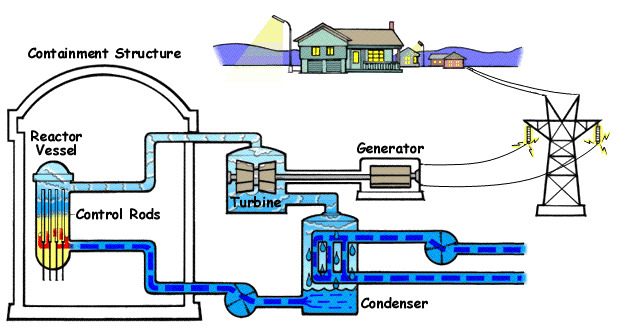
\includegraphics[width=\linewidth]{Images/bwr.jpg}
              \end{minipage}
            \end{center}
      \item PWR (\emph{Pressurized Water Reactor}):
            \begin{center}
              \begin{minipage}{\linewidth}
                \centering
                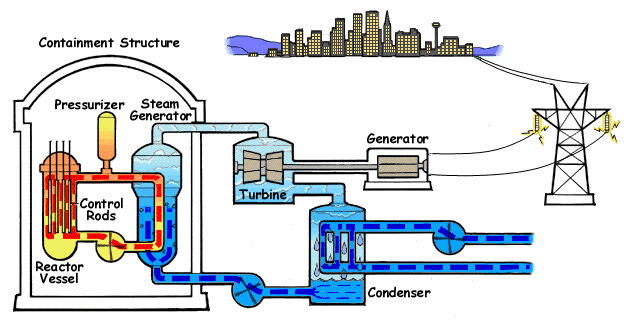
\includegraphics[width=\linewidth]{Images/pwr.jpg}
              \end{minipage}
            \end{center}
    \end{enumerate}
  \end{definition}
  \begin{definition}[Nuclear fusion]
    \emph{Nuclear fusion} is a reaction in which two or more atomic nuclei are combined to form one or more different atomic nuclei and subatomic particles (neutrons or protons)\footnote{Even that nuclear fusion is still being the energetic promise of the future, its production is very costly. Indeed, we have to put together the nuclei in the way that the strong interaction overcome the electrostatic force, that is, put the nuclei together at a distance of $\sim 10^{-15}\text{ m}$.}. The most interesting fusion reactions are:
    \begin{align*}
      \ce{^2H}+\ce{^2H} & \rightarrow\text{n}+\ce{^3He}\qquad & (Q=3.3\text{ MeV})  \\
      \ce{^2H}+\ce{^2H} & \rightarrow\text{p}+\ce{^3H}\qquad  & (Q=4.0\text{ MeV})  \\
      \ce{^2H}+\ce{^1H} & \rightarrow\ce{^3He}+\gamma\qquad   & (Q=5.49\text{ MeV}) \\
      \ce{^2H}+\ce{^3H} & \rightarrow\text{n}+\ce{^4He}\qquad & (Q=17.6\text{ MeV})
    \end{align*}
  \end{definition}
  \subsubsection{Elementary particles}
  \begin{definition}[Elementary particles]
    All the matter is composed by 12 fermions (6 quarks and 6 leptons) and all of these have an associated antiparticle. Quarks and Leptons can interact with each other by exchanging Gauge bosons which are carriers of the 4 fundamental forces.
  \end{definition}
  \begin{definition}[Antimatter]
    Each elementary particle has an associated \emph{antiparticle} which has the same properties as the initial particle but has different sign on all the charges.
  \end{definition}
  \begin{definition}[Quark]
    A \emph{quark} is a fermion with fractional electric charge by 1/3. There are 6 types of quarks, known as \emph{flavors}: \emph{up} $u$ and \emph{down} $d$ (first generation); \emph{charm} $c$ and \emph{strange} $s$ (second generation), and \emph{top} $t$ and \emph{bottom} $b$ (third generation)\footnote{An important fact of quarks is that they cannot be isolated due to the \emph{color confinement} property (see definition \cref{SMT_color}).}.
  \end{definition}
  \begin{definition}[Lepton]
    A \emph{lepton} is a fermion which does not undergo strong interaction. There are 6 types of leptons, known as \emph{flavors}: \emph{electron} $e^-$ and \emph{electron neutrino} $\nu_e$ (first generation); \emph{muon} $\mu^-$ and \emph{muon neutrino} $\nu_\mu$ (second generation), and \emph{tau} $\tau^-$ and \emph{tau neutrino} $\nu_\tau$ (third generation).
  \end{definition}
  \begin{definition}[Lepton number]
    \emph{Lepton number} $L$ is a quantum number that is conserved in all interactions. It is defined as: $$L=n_\ell-n_{\bar{\ell}}$$ where where  $n_\ell$ is the number of leptons and $n_{\bar{\ell}}$ is the number of antileptons in a reaction. In addition to lepton number, \emph{lepton family numbers} are defined as:
    \begin{itemize}
      \item \emph{Electron number} $L_e$: for the electron and electron neutrino.
      \item \emph{Muon number} $L_\mu$: for the muon and muon neutrino.
      \item \emph{Tau number} $L_\tau$: for the tau and tau neutrino.
    \end{itemize}
    These numbers are also preserved during collisions.
    \begin{center}
      \begin{minipage}{\linewidth}
        \centering
        \begin{tabular}{cccc}
                           & $L_e$ & $L_\mu$ & $L_\tau$ \\
          \hline
          $e^-$            & $+1$  & 0       & 0        \\
          $\nu_e$          & $+1$  & 0       & 0        \\
          $e^+$            & $-1$  & 0       & 0        \\
          $\bar{\nu}_e$    & $-1$  & 0       & 0        \\
          $\mu^-$          & 0     & $+1$    & 0        \\
          $\nu_\mu$        & 0     & $+1$    & 0        \\
          $\mu^+$          & 0     & $-1$    & 0        \\
          $\bar{\nu}_\mu$  & 0     & $-1$    & 0        \\
          $\tau^-$         & 0     & 0       & $+1$     \\
          $\nu_\tau$       & 0     & 0       & $+1$     \\
          $\tau^+$         & 0     & 0       & $-1$     \\
          $\bar{\nu}_\tau$ & 0     & 0       & $-1$     \\
        \end{tabular}
        \captionof{table}{Lepton family numbers}
      \end{minipage}
    \end{center}
  \end{definition}
  \begin{definition}[Hadron]
    A \emph{hadron} is a subatomic particle made of two or three quarks held together by the strong force. There are two types of hadrons:
    \begin{itemize}
      \item Baryons: made of three quarks.
      \item Mesons: made of two quarks.
    \end{itemize}
  \end{definition}
  \begin{definition}[Color charge]\label{SMT_color}
    The \emph{color charge}\footnote{The color charge of quarks and gluons is completely unrelated to the everyday meaning of color.} is a property of quarks and gluons (see \cref{SMT_interactions}) that is related to the particles' strong interactions. There are three types of colors (\emph{red}, \emph{green} and \emph{blue}) and three types of anticolors (\emph{antired}, \emph{antigreen} and \emph{antiblue}). This two families of colors mixed together, or one color with its anticolor, produces the color \emph{white} or, equivalently, has a net color charge of zero.
  \end{definition}
  \begin{definition}[Fundamental interactions]\label{SMT_interactions}
    Fundamental interactions are characterized by the exchange of bosons. The 4 fundamental interactions are:
    \begin{itemize}
      \item Electromagnetic interaction: Based on emission and absorption of photons. The particles with which it interacts have nonzero electric charge. This interaction is described by quantum electrodynamics (QED).
      \item Strong interaction: It is transported by gluons. The particles with which it interacts have nonzero color charge. This interaction is described by quantum chromodynamics (QCD)\footnote{In particular, strong interaction is the responsible of maintaining the atomic nucleus unified: since protons have charge $+e$, they experience an electric force that tends to push them apart, but at short range ($\sim10^{-15}\text{ m}$) the attractive nuclear force is strong enough to overcome the electromagnetic force.}.
      \item Weak interaction: It is transported by bosons $W^+$, $W^-$ and $Z^0$. It modifies the flavour of a particle.
      \item Gravity: Te particles wit which it interacts have nonzero mass. The carrier particle of this forces is the graviton, which hasn't been observed yet.
    \end{itemize}
    \begin{center}
      \begin{minipage}{\linewidth}
        \centering
        \begin{tabular}{lcc}
          \hline
          \hline
          Interaction     & Relative intensity & Boson                   \\
          \hline
          Strong          & 1                  & Gluon $g$               \\
          Electromagnetic & $10^{-2}$          & Photon $\gamma$         \\
          Weak            & $10^{-7}$          & $W^+\quad W^-\quad Z^0$ \\
          Gravitational   & $10^{-39}$         & Graviton $G$            \\
          \hline
          \hline
        \end{tabular}
        \captionof{table}{Relative intensity of fundamental forces}
      \end{minipage}
    \end{center}
  \end{definition}
  \begin{definition}[Grand Unified Theory]
    Electromagnetic and weak forces join together in a unique \emph{electroweak theory} for energies $\gg 100\text{ GeV}$. This one join with strong force in the \emph{Grand Unified Theory} for energies $\sim 10^{15}\text{ GeV}$. And finally, the 4 interaction join together at energies $>10^{20}\text{ GeV}$ or distances $\sim 10^{-34}\text{ m}$.
  \end{definition}
  \subsubsection{Solids}
  \begin{definition}
    A solid is \emph{crystalline} if atoms form a regular and structured patron. A solid is \emph{amorphous} if the arrangement of atoms is not regular.
  \end{definition}
  \begin{proposition}[Classical interpretation of resistivity]
    Consider a metal of resistivity $\rho$ with $n_e$ electrons per unit of volume moving at an average speed of $v_\text{av}$. Then: $$\rho=\frac{m_ev_\text{av}}{n_ee^2\lambda}$$ where $\lambda=v_\text{av}\tau$ is the mean free path of electrons between collisions with the lattice ions and $\tau$ is the average time between these collisions\footnote{We know that $\rho\propto v_\text{av}\propto\sqrt{T}$ but empirically it is observed that $\rho\propto T$. The classical model is, therefore, inconsistent.}.
  \end{proposition}
  \begin{proposition}[Quantum interpretation of resistivity]
    Free electrons do not interact neither with ions nor with themselves. Indeed they behave as a particles in a gas (\emph{fermi gas}). Moreover by Pauli exclusion principle, there can only be two electrons in each energy state. At $T=0\text{ K}$ the energy $E_F$ of the last filled (or half-filled) energy state is called \emph{Fermi energy}: $$E_F=\frac{h^2}{8m_e}{\left(\frac{3N}{\pi V}\right)}^{2/3}$$ where $N$ is the number of free electrons and $V$ is the volume they occupy. That is, $\frac{N}{V}$ is the density of free electrons. The average energy $E_\text{av}$ at $T=0\text{ K}$ is: $$E_\text{av}=\frac{3}{5}E_F$$
  \end{proposition}
  \begin{definition}
    The \emph{Fermi factor} $f(E)$ is defined as the probability of a state being occupied. At $T=0\text{ K}$ we have: $$f(E)=
      \begin{cases}
        1 & \text{if }E<E_F \\
        0 & \text{if }E>E_F
      \end{cases}
    $$
    If $T\ne 0\text{ K}$ some electrons gain enough energy to level up and therefore we should redefine $E_F$ in the following way: energy in which the probability of its corresponding state being occupied is 1/2. Therefore the Fermi factor becomes:
    \begin{center}
      \begin{minipage}{\linewidth}
        \centering
        \includestandalone[mode=image|tex,width=0.5\linewidth]{Images/fermi}
      \end{minipage}
    \end{center}
  \end{definition}
  \begin{proposition}[Band Theory of Solids]
    When many atoms are brought together to form a solid, the individual energy levels are split into bands of allowed energies. The splitting depends on the type of bonding and the lattice separation. The highest energy band that contains electrons is called the \emph{valence band} (\emph{VB}). The lowest energy band that is not filled with electrons is called the \emph{conduction band} (\emph{CB}).
    \begin{center}
      \begin{minipage}{\linewidth}
        \centering
        \includestandalone[mode=image|tex,width=\linewidth]{Images/band_theory}
        \captionof{figure}{Band of levels on a conductor, insulator and semiconductor. In red there are the levels occupied by electrons and in green the levels empty.}
      \end{minipage}
    \end{center}
    \begin{itemize}
      \item In a conductor, the valence band is only partially filled, so there are many available empty energy states for excited electrons which can move freely through these states.
      \item In an insulator, the valence band is completely filled and there is a large energy gap between it and the next allowed band, the conduction band. Therefore, the electrons can barely move.
      \item In a semi-conductor, the energy gap between the filled valence band and the empty conduction band is small; so, at ordinary temperatures, an appreciable number of electrons are thermally excited into the conduction band.
    \end{itemize}
  \end{proposition}
\end{multicols}
\begin{center}
  \begin{minipage}{\linewidth}
    \centering
    \includestandalone[mode=image|tex,width=0.75\linewidth]{Images/standard_model}
  \end{minipage}
\end{center}
\begin{multicols}{2}
  \subsection{Heat transfer}
  \begin{definition}[Heat]
    The \emph{heat} is the transport of thermal energy due to the temperature difference. The fundamental modes of heat transfer are: \emph{conduction}, \emph{convection} and \emph{radiation}.
  \end{definition}
  \subsubsection{Conduction}
  \begin{definition}[Conduction]
    \emph{Thermal conduction} is the heat transfer produced by the contact of two object at different temperatures in the absence of matter transfer. Microscopically, energy is transferred throughout the material due to collisions of particles and the movement of electrons within the body.
  \end{definition}
  \begin{law}[Fourier's law]
    The law of heat conduction states that
    $$\grad\vf{\Phi}_q=-\lambda\grad T$$ where $\vf{\Phi}_q$ is the heat flux density (energy transferred per unit of surface and time) and $\lambda$ is the material's \emph{thermal conductivity} ($[\lambda]=\text{W}\cdot\text{m}^{-1}\cdot\text{K}^{-1}$).
  \end{law}
  \begin{proposition}[Heat equation]
    For a medium at a temperature $T(\vf{r},t)$ we have:
    $$\pdv{T}{t}=\frac{\lambda}{\rho c_s}\laplacian T=:\alpha\laplacian T$$
    where $\rho$ is the density of the material; $c_s$, its specific heat capacity; $\lambda$, its thermal conductivity, and $\alpha$ its \emph{thermal diffusivity}.
  \end{proposition}
  \begin{law}[Fick's law]
    The solute in a solvent at rest will move from a region of high concentration to a region of low concentration across a concentration gradient. Mathematically, if $\vf{J}$ is the diffusion flux; $D$, the diffusion coefficient, and $c$, the concentration, then:
    $$\vf{J}=-D\grad c$$
  \end{law}
  \begin{proposition}[Diffusion equation]
    The diffusion equation is: $$\pdv{c}{t}=D\laplacian c$$
  \end{proposition}
  \begin{proposition}
    Suppose that inside a material there is a source of heat which generates an amount of heat $\dot{q}$ per unit of volume and time. Then:
    $$\rho c_s\pdv{T}{t}=\lambda\laplacian T+\dot{q}$$
    where $\rho$ is the density of the material; $c_s$, its specific heat capacity, and $\lambda$, its thermal conductivity.
    For the case of creating matter instead of energy and measuring the solute $c$ of the solvent we have:
    $$\pdv{c}{t}=D\laplacian c+f(c,t)$$
    where $D$ is the diffusion coefficient and $f(c,t)$ is the function that measures the net solute created and destructed per unit of volume and time.
  \end{proposition}
  \subsubsection{Convection}
  \begin{definition}[Convection]
    \emph{Thermal convection} is the heat transfer from one place to another due to the movement of fluid.
  \end{definition}
  \begin{proposition}[Newton's law of cooling]
    A body subjected to a forced convection exchanges heat with its surroundings as: $$\dv{q}{t}=hA(T-T_0)$$ where $h$ is the \emph{heat transfer coefficient}; $A$, the heat transfer surface area; $T$, the temperature of the body on its surface, and $T_0$, the temperature of the environment.
  \end{proposition}
  \subsubsection{Radiation}
  \begin{definition}[Radiation]
    \emph{Thermal radiation} is the emission of electromagnetic waves from all matter that has a temperature greater than absolute zero. Moreover, the power radiated from an object in a vacuum is: $$P=\varepsilon\sigma T^4$$ where $0<\varepsilon<1$ is the emissivity of the object;$\sigma$, the Stefan-Boltzmann constant, and $T$, the temperature of the object.
  \end{definition}
  \subsection{Thermodynamics}
  \subsubsection{Basic definitions}
  \begin{definition}[Thermodynamic system]
    A \emph{thermodynamic system} is a region of the universe confined by walls. There are three types of systems:
    \begin{itemize}
      \item \emph{Open system}: can exchange energy and matter with its surroundings (made of permeable and diathermic walls).
      \item \emph{Closed system}: can exchange energy with its surroundings but not matter (made of impermeable and diathermic walls).
      \item \emph{Isolated system}: can exchange neither energy nor matter with its surroundings (made of impermeable and adiabatic walls).
    \end{itemize}
  \end{definition}
  \begin{definition}
    Variables which measure the macroscopic measurable properties of the state of a system are called \emph{state variables} and can be of two types:
    \begin{enumerate}
      \item \emph{Extensive}: are additive and scale the size of the system. Examples of such variables are: mass, volume, energy...
      \item \emph{Intensive}: do not depend on the system size or the amount of material in the system. Examples of such variables are: temperature, density, pressure...
    \end{enumerate}
    Moreover, \emph{specific variables} are those created from an extensive variable and divided by the volume, number of moles, mass... Examples of such variables are: specific volume, density, specific heat capacity...
  \end{definition}
  \begin{definition}
    A system is in
    \begin{enumerate}
      \item \emph{mechanical equilibrium} if the net force acting on the system is zero.
      \item \emph{thermal equilibrium} if there is no net flow of thermal energy inside it or between it and its surroundings.
      \item \emph{chemical equilibrium} if there are no chemical reactions on the system.
      \item \emph{thermodynamical equilibrium} if it is in mechanical, thermal and chemical equilibrium simultaneously.
    \end{enumerate}
  \end{definition}
  \begin{definition}
    There are different types of equilibrium:
    \begin{itemize}
      \item \emph{Stable}: after a slight disturbance, the system returns to the equilibrium.
      \item \emph{Unstable}: after a slight disturbance, the system get away from the equilibrium.
      \item \emph{Metastable}: after a slight disturbance, the system returns to the equilibrium but if the disturbance is strong enough the system may get away from the equilibrium.
      \item \emph{Neutral}: a slight disturbance does not displace the system from the equilibrium.
    \end{itemize}
    \begin{center}
      \begin{minipage}{0.24\linewidth}
        \centering
        \includestandalone[mode=image|tex,width=\linewidth]{Images/equilibrium_stab}
        \captionof*{figure}{Stable}
      \end{minipage}
      \begin{minipage}{0.24\linewidth}
        \centering
        \includestandalone[mode=image|tex,width=\linewidth]{Images/equilibrium_unstab}
        \captionof*{figure}{Unstable}
      \end{minipage}
      \begin{minipage}{0.24\linewidth}
        \centering
        \includestandalone[mode=image|tex,width=\linewidth]{Images/equilibrium_meta}
        \captionof*{figure}{Metastable}
      \end{minipage}
      \begin{minipage}{0.24\linewidth}
        \centering
        \includestandalone[mode=image|tex,width=\linewidth]{Images/equilibrium_neutr}
        \captionof*{figure}{Neutral}
      \end{minipage}
    \end{center}
  \end{definition}
  \begin{definition}[Thermodynamic process]
    A \emph{thermodynamic process} is the passage between two states of equilibrium. We distinguish the following types of processes:
    \begin{itemize}
      \item \emph{Quasi-static process}: the system passes through states infinitely close to the equilibrium.
            \begin{itemize}
              \item \emph{Reversible process}: the system can be inverted in each infinitesimally step by changing the sign of the external parameters.
              \item \emph{Irreversible process}: the system cannot be inverted in each infinitesimally step by changing the sign of the external parameters.
            \end{itemize}
      \item \emph{Non-quasi-static process}: the system passes through non-equilibrium states.
    \end{itemize}
  \end{definition}
  \subsubsection{Zeroth law of thermodynamics}
  \begin{definition}
    We say that two systems are in \emph{thermal contact} if they are separated by a diathermic wall.
  \end{definition}
  \begin{law}[Zeroth law of thermodynamics]
    If two systems are both in thermal equilibrium with a third system, then they are in thermal equilibrium with each other.
  \end{law}
  \begin{corollary}
    Being in thermal equilibrium is an equivalence relation.
  \end{corollary}
  \begin{definition}
    The \emph{empirical temperature} is a common state variable between the systems that are in thermal equilibrium.
  \end{definition}
  \begin{proposition}
    The conversions between Celsius, Fahrenheit and Kelvin scales are:
    $$T(^\circ\text{C})=\frac{5}{9}\left(T(^\circ\text{F})-32\right)\qquad T(^\circ\text{C})=T(^\circ\text{K})-273.15$$
  \end{proposition}
  \begin{proposition}
    Let $z=z(x,y)$ be a function. Then:
    $$\left(\pdv{z}{y}\right)_x=\frac{1}{\left(\pdv{y}{z}\right)_x}\qquad\left(\pdv{z}{x}\right)_y=-\left(\pdv{z}{y}\right)_x\left(\pdv{y}{x}\right)_z$$
  \end{proposition}
  \begin{definition}[Thermal expansion]
    The \emph{volumetric coefficient of thermal expansion} is given by
    $$\alpha:=\alpha_\text{V}=\frac{1}{V}\left(\pdv{V}{T}\right)_p$$
    where the subscript $p$ indicates that the pressure is held constant during the process.
  \end{definition}
  \begin{definition}[Compressibility]
    \emph{Isothermal compressibility} is defined as
    $$\kappa_T=-\frac{1}{V}\left(\pdv{V}{p}\right)_T$$
    where the subscript $T$ indicates that the temperature is held constant during the process.
  \end{definition}
  \begin{definition}[Thermal pressure]
    The \emph{thermal pressure coefficient} is defined as:
    $$\beta=\left(\pdv{P}{T}\right)_V=\frac{\alpha}{\kappa_T}$$
    where the subscript $V$ indicates that the volume is held constant during the process.
  \end{definition}
  \subsubsection{Work}
  \begin{definition}
    The work done by a hydrostatic system is: $$\dd{W}=-p\dd{V}\implies W=-\int_{V_\text{i}}^{V_\text{f}}p\dd{V}$$ where $V_\text{i}$ and $V_\text{f}$ are the initial and final volumes of the system, respectively.
  \end{definition}
  \begin{lemma}[Sign convention of work]
    Given a system we have:
    \begin{itemize}
      \item $W>0$, if the surroundings of the system do work on the system.
      \item $W<0$, if the system do work on its surroundings.
    \end{itemize}
  \end{lemma}
  \begin{proposition}
    Depending on the type of process, we get different values for the total work done on the process:
    \begin{itemize}
      \item Isochoric process ($V=\text{const.}$):
            $$\dd{V}=0\implies W=0$$
      \item Isobaric process ($p=\text{const.}$):
            $$W=-p\Delta V$$
            where $p$ is the pressure of the system and $\Delta V$ is the difference of volume between the initial and final states.
      \item Isothermal process ($T=\text{const.}$):
            $$W=-nRT\ln\left(\frac{V_\text{f}}{V_\text{i}}\right)$$
            where $n$ is the number of moles of present gas, $R$ is the ideal gas constant, $T$ is the temperature of the system and $V_\text{i}$ and $V_\text{f}$ are the initial and final volumes of the system, respectively.
    \end{itemize}
  \end{proposition}
  \subsubsection{First law of thermodynamics}
  \begin{law}[First law of thermodynamics in isolated systems]
    In an isolated system, the work done by a process between two arbitrary states is independent of that process and depends only on the initial and final states.
  \end{law}
  \begin{corollary}
    We define the \emph{internal energy} $U_B$ of the state $B$ as:
    $$U_B=U_A+W_{A\to B}^\text{ad}\implies \Delta U=W_{A\to B}^\text{ad}$$
    where $U_A$ is the internal energy of the state $A$, and $W_{A\to B}^\text{ad}$ is the work done to go form $A$ to $B$ through an adiabatic process.
  \end{corollary}
  \begin{law}[First law of thermodynamics in closed systems]
    In a closed system, the work done to go from an initial state to a final state does depend on the process followed and not only on the initial and final states.
  \end{law}
  \begin{corollary}
    In a closed system, we define the \emph{heat supplied to the system} $Q$ in a process between two states $A$ and $B$ as:
    $$Q_{A\to B}=\Delta U-W_{A\to B}$$
    Or in differential form:
    $$\delta Q=\dd{U}-\delta W$$
    where $\delta$ is not exactly the differential of a function.
  \end{corollary}
  \begin{lemma}[Sign convention of heat]
    Given a system we have:
    \begin{itemize}
      \item $Q>0$, if the heat is added to the system.
      \item $Q<0$, if the heat is rejected from the system.
    \end{itemize}
  \end{lemma}
  \begin{definition}
    Relating the heat capacity of a substance we have: $$C_X=\dv{Q_X}{T}$$
    where the subscript $X$ indicates that the variable $X$ is held constant during the expansion.
  \end{definition}
  \begin{definition}
    \emph{Latent heat} is the amount of heat required to completely change the phase of a kilogram of a substance.
  \end{definition}
  \begin{definition}[Enthalpy]
    We define the \emph{enthalpy} $H$ of a system as: $$H=U+pV$$
    where $U$ is the internal energy, $p$ is the pressure and $V$ is the volume.
  \end{definition}
  \begin{proposition}
    Relating the heat capacities $C_V$ and $C_p$ holding constant the volume and the pressure, respectively, we have:
    $$C_V=\left(\pdv{U}{T}\right)_V\qquad C_p=\left(\pdv{H}{T}\right)_p$$
    And in general:
    $$C_p=C_V+\left[\left(\pdv{U}{V}\right)_T+p\right]\left(\dv{V}{T}\right)_p$$
  \end{proposition}
  \begin{proposition}[Reversible adiabatic equation for an ideal gas]
    The equation for an ideal gas undergoing a reversible adiabatic process is:
    \begin{align*}
      \dd{U}+p\dd{V}=0 & \implies nc_V\dd{T}+\frac{nRT}{V}\dd{V}=0 \\
                       & \implies\left\{
      \begin{aligned}
        pV^\gamma            & =\const \\
        V^{\gamma-1} T       & =\const \\
        p^{1-\gamma}T^\gamma & =\const
      \end{aligned}\right.
    \end{align*}
  \end{proposition}
  \subsubsection{Second law of thermodynamics}
  \begin{law}[Second law of thermodynamics]
    No system can absorb heat from a single reservoir and convert it entirely into work without additional net changes in the system or its surroundings.
  \end{law}
  \begin{definition}
    A \emph{heat engine} is a cyclic device whose purpose is to convert as much heat into work as possible. Heat engines contain a working substance (water in a steam engine) that absorbs a quantity of heat $Q_\text{h}$ (hot) from a high temperature reservoir, does work $W$ on its surroundings, and releases heat $Q_\text{c}$ (cool) as it returns to its initial state.
    Its efficiency $\eta$ is given by: $$\eta=\frac{W}{Q_\text{h}}=1-\frac{Q_\text{c}}{Q_\text{h}}$$
  \end{definition}
  \begin{definition}
    A \emph{refrigerator engine} absorbs heat $Q_\text{c}$ (cold) from the interior of a refrigerator and releases heat $Q_\text{h}$ (hot) to the surroundings. This process requires work $W$ to be done on the refrigerator.
    Its efficiency $\eta$ is given by: $$\eta=\frac{Q_\text{c}}{W}$$
  \end{definition}
  \begin{definition}
    A \emph{heat pump} is a refrigerator with a different objective. It absorbs heat $Q_\text{c}$ from the outside (cold reservoir) and releases heat $Q_\text{h}$ into the object or region of interest. This process requires work $W$ to be done on the heat pump.
    Its efficiency $\eta$ is given by: $$\eta=\frac{Q_\text{h}}{W}$$
  \end{definition}
  \begin{center}
    \begin{minipage}{0.49\linewidth}
      \centering
      \includestandalone[mode=image|tex,width=0.75\linewidth]{Images/heat_engine}
      \captionof{figure}{Heat engine}
    \end{minipage}\hfill
    \begin{minipage}{0.49\linewidth}
      \centering
      \includestandalone[mode=image|tex,width=0.75\linewidth]{Images/heat_pump}
      \captionof{figure}{Heat pump}
    \end{minipage}
  \end{center}
  \begin{definition}[Carnot cylce]
    \emph{Carnot cycle} is a reversible thermodynamic process that consists of the following steps:
    \begin{enumerate}
      \item Isothermal expansion
      \item Adiabatic expansion
      \item Isothermal compression
      \item Adiabatic compression
    \end{enumerate}
    The efficiency $\eta_\text{C}$ of Carnot cycle is:
    $$\eta_\text{C}=1-\frac{T_\text{c}}{T_\text{h}}$$
    where $T_\text{h}$ and $T_\text{c}$ are the temperatures at the isothermal processes (see \cref{carnot}). Moreover it is satisfied that: $$\frac{Q_\text{c}}{Q_\text{h}}=\frac{T_\text{c}}{T_\text{h}}$$
    \begin{center}
      \begin{minipage}{\linewidth}
        \centering
        \includestandalone[mode=image|tex,width=0.8\linewidth]{Images/carnot}
        \captionof{figure}{Carnot cycle}
        \label{SMT_carnot}
      \end{minipage}
    \end{center}
  \end{definition}
  \begin{theorem}[Carnot's theorem]
    All heat engines between two heat reservoirs are less or equally efficient than a Carnot heat engine operating between the same reservoirs.
  \end{theorem}
  \begin{corollary}
    All reversible machines working between two heat reservoirs has the same efficiency.
  \end{corollary}
  \begin{proposition}
    Consider a machine that realizes a Carnot cycle. Let $T_1$ and $T_2$ be the temperatures of the two reservoirs and $T_{1,\text{w}}$ and $T_{2,\text{w}}$ the temperatures of the machine when it is in touch with reservoirs of temperatures $T_1$ and $T_2$, respectively. Then, the power of this cycle\footnote{In a reversible cycle the efficiency is maximum but because of it is extremely slow the power is null. } is:
    $$P=\lambda\frac{(T_1-T_{1,\text{w}})(T_{2,\text{w}}-T_2)(T_{1,\text{w}}-T_{2,\text{w}})}{T_1(T_1-T_{1,\text{w}})+T_2(T_{2,\text{w}}-T_2)}$$
    where $\lambda$ is the material’s conductivity. The efficiency when the power is maximum is:
    $$\eta=1-\sqrt{\frac{T_2}{T_1}}<\eta_\text{C}$$
  \end{proposition}
  \subsubsection{Entropy}
  \begin{theorem}[Clausius theorem]
    For a thermodynamic system exchanging heat with external reservoirs and undergoing a thermodynamic cycle we have:
    $$\oint\frac{\delta Q}{T}\leq 0$$
    where $\delta Q$ is the heat exchange with a reservoir at a temperature $T$. Moreover if the cycle is reversible, we have:
    $$\oint\frac{\delta Q_\text{rev}}{T}=0$$
  \end{theorem}
  \begin{definition}[Entropy]
    There exists a new state function, called \emph{entropy} $S$, such that:
    $$S(B)-S(A)=\int_A^B\frac{\delta Q_\text{rev}}{T}\quad\text{or}\quad\dd{S}=\frac{\delta Q_\text{rev}}{T}$$
  \end{definition}
  \begin{law}[Second law of thermodynamics in terms of entropy]
    In an isolated system, the entropy cannot decrease: $\Delta S\geq 0$. Moreover: $${\Delta S}_\text{universe}={\Delta S}_\text{system}+{\Delta S}_\text{surroundings}\geq 0$$
  \end{law}
  \begin{proposition}
    Entropy in different processes:
    \begin{itemize}
      \item Cyclic process: $$\Delta S=0$$
      \item Reversible adiabatic process: $$\Delta S=0$$
      \item Reversible isothermal process at temperature $T$: $$\Delta S=\frac{Q}{T}$$ where $Q$ is the heat exchanged on the process.
      \item Thermal contact between two reservoirs at temperatures $T_1$ and $T_2$: $$\Delta S=Q\left(\frac{1}{T_2}-\frac{1}{T_1}\right)$$ where $Q$ is the heat exchanged on the process.
      \item Change on temperature at constant volume: $$\Delta S=C_V\ln\frac{T_2}{T_1}$$ where $T_1$ is the initial temperature and $T_2$ the final temperature.
      \item Change on temperature at constant pressure: $$\Delta S=C_p\ln\frac{T_2}{T_1}$$ where $T_1$ is the initial temperature and $T_2$ the final temperature.
      \item Free adiabatic expansion of an ideal gas: $$\Delta S=nRT\ln\frac{V_2}{V_1}$$ where $V_1$ is the initial volume and $V_2$ the final volume.
      \item Arbitrary process of an ideal gas: $$\Delta S=nRT\ln\frac{V_2}{V_1}+nc_p\ln\frac{T_2}{T_1}$$
    \end{itemize}
  \end{proposition}
  \begin{definition}
    We define the \emph{Helmholtz free energy} $F$ as:
    $$F=U-TS$$
    At equilibrium, Helmholtz free energy is minimized.
  \end{definition}
  \begin{definition}
    We define the \emph{Gibbs free energy} $G$ as:
    $$G=H-TS$$
  \end{definition}
  \begin{proposition}
    2nd law of thermodynamics applied to non-isolated systems: $$\Delta G=\Delta U+p\Delta V-T\Delta S\leq 0$$
  \end{proposition}
  \begin{proposition}
    For a non-isolated system, we have different criteria to know whether or not a the system is spontaneous.
    \begin{itemize}
      \item If $T,p=\text{const.}$, then $\Delta G\leq 0$.
      \item If $T,V=\text{const.}$, then $\Delta F\leq 0$.
      \item If $S,p=\text{const.}$, then $\Delta H\leq 0$.
      \item If $S,V=\text{const.}$, then $\Delta U\leq 0$.
      \item If $U,V=\text{const.}$, then $\Delta S\geq 0$.
    \end{itemize}
  \end{proposition}
  \begin{proposition}
    The maximum amount of work that the system can perform in a thermodynamic process in which temperature is held constant is $|\Delta F|$.
  \end{proposition}
  \begin{proposition}[Gibbs equation]
    For a closed system we have: $$\dd{U}=T\dd{S}-p\dd{V}$$
    For an open system we have: $$\dd{U}=T\dd{S}-p\dd{V}+\mu\dd{N}$$
    where $\mu$ is the chemical potential and $N$ is the number of particles in the system.
  \end{proposition}
\end{multicols}
\end{document}